\documentclass[12pt, letterpaper]{report}
\usepackage{graphicx}
\usepackage{hyperref}
\usepackage{amssymb}
\usepackage{amsmath}
\usepackage{float}
\usepackage{mathtools}
\usepackage{enumitem}
\usepackage[margin=1in]{geometry}
\usepackage[figurename=Figura]{caption}
\title{Actividad: Análisis de circuitos eléctricos}
\author{Juan Pablo Guerrero Escudero, A01706810}
\date{22 abril, 2024}
\begin{document}
\maketitle
\subsection*{Cálculo para determinar voltajes}
En la actividad, se tiene la tarea de determinar los voltajes del siguiente circuito: 
\begin{figure}[H]
    \centering
    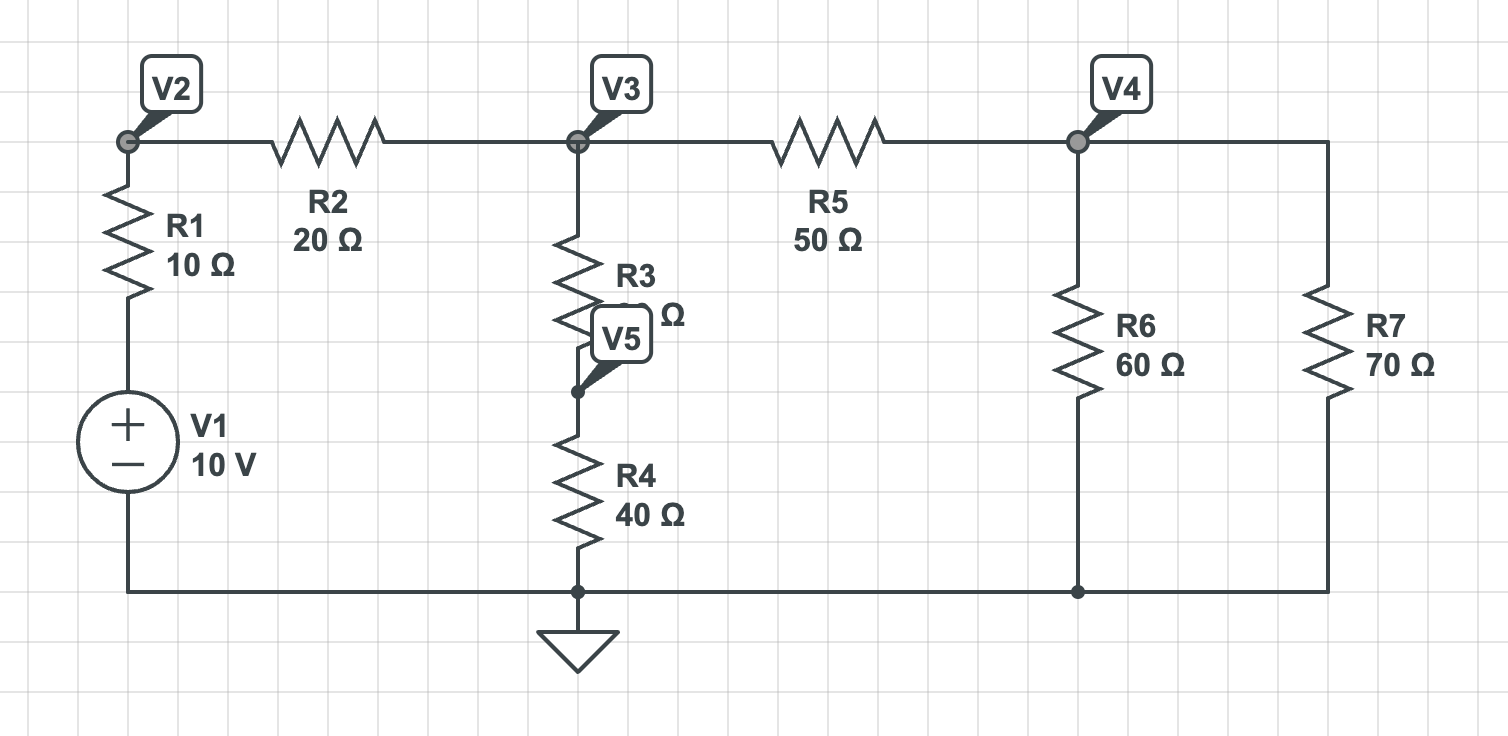
\includegraphics[height = 6cm]{2024-04-22_DiagramaActividadCircuito.png}
    \caption{Diagrama del circuito}
\end{figure}
En primer lugar, se tienen 4 nodos (V1, V2, V3, V4) debido a que el nodo entre V1 y r1 resulta de $V = 10v$ porque 
al estar conectado a la parte positiva de la batería, y la parte negativa de ésta está conectada a Tierra, el voltaje del nodo 
es igual al voltaje de la pila. \\ 
En segundo lugar, se tienen 5 nodos, pero como el primero ya está resuelto, quedan 4 nodos, por lo cuál se forma un sistema de ecuaciones de tamaño 
$(4X4)$, que es cuadrado. Para hacer la planteación de las ecuaciones nodales, se toma en cuenta la Ley de Kirchoff, que dice: "La suma de todas las corrientes 
que fluyen hacia afuera del nodo es igual a cero", es decir, la corriente que entra es igual a la corriente que sale de cada nodo. Por último, para el cálculo de 
cada corriente tomamos en cuenta la Ley de Ohm, que dice $V = RI $, y despejando para la corriente resulta $I = \frac{V}{R}$, siendo $V$ la diferencia de voltaje en cada nodo. \\

Por lo tanto, se plantea el sistema de ecuaciones de la siguiente manera: 
\begin{align}
\frac{V_2 - V_1}{R_1} + \frac{V_2 - V_3}{R_2} &= 0\\ 
\frac{V_3 - V_2}{R_2} + \frac{V_3 - V_5}{R_3} + \frac{V_3 - V_4}{R_5} &= 0\\ 
\frac{V_4 - V_3}{R_5} + \frac{V_4 - 0}{R_6} + \frac{V_4 - 0}{R_7} &= 0\\
\frac{V_5 - V_3}{R_3} + \frac{V_5 - 0}{R_4} &= 0
\end{align}
Si factorizamos por medio de los términos comúnes, el sistema anterior se reescribe de la siguiente manera: 
\begin{align}
V_2(\frac{1}{R_1} + \frac{1}{R_2}) - V_3(\frac{1}{R_2}) &= \frac{V_1}{R_1}\\
-V_2(\frac{1}{R_2}) + V_3(\frac{1}{R_2} + \frac{1}{R_3} + \frac{1}{R_5}) - V_4(\frac{1}{R_5}) - V_5(\frac{1}{R_3}) &= 0\\ 
-V_3(\frac{1}{R_5}) + V_4(\frac{1}{R_5} + \frac{1}{R_6} + \frac{1}{R_7}) &= 0\\ 
-V_3(\frac{1}{R_3}) + V_5(\frac{1}{R_3} + \frac{1}{R_4}) &= 0
\end{align}
Desde aquí, podemos escribir éste sistema como una ecuación matricial de la forma $A\vec{x} = \vec{b}$, donde $A$ es la 
matriz de coeficientes, $\vec{x}$ es el vector de incógnitas, y $\vec{b}$ es el vector del lado derecho. 
\begin{align}
A &= \begin{bmatrix}
\frac{1}{R_1} + \frac{1}{R_2} & -\frac{1}{R_2} & 0 & 0\\
-\frac{1}{R_2} & \frac{1}{R_2} + \frac{1}{R_3} + \frac{1}{R_5} & -\frac{1}{R_5} & -\frac{1}{R_3}\\ 
0 & -\frac{1}{R_5} & \frac{1}{R_5} + \frac{1}{R_6} + \frac{1}{R_7} & 0\\
0 & -\frac{1}{R_3} & 0 & \frac{1}{R_3} + \frac{1}{R_4}
\end{bmatrix}\\
\vec{x} &= \begin{bmatrix}
V_2 \\ 
V_3 \\ 
V_4 \\
V_5
\end{bmatrix}\\
\vec{b} &= \begin{bmatrix}
    \frac{V_1}{R_1} \\
    0 \\
    0 \\
    0
\end{bmatrix}
\end{align} Para obtener el vector de la solución de las incógnitas, se utiliza Matlab, y el comando \begin{verbatim}
x = A\B
\end{verbatim}el cual resuelve el sistema de ecuaciones lineales de la forma $A \vec{x} = \vec{b}$, siempre y cuando 
el número de columnas de $A$ sea igual al número de filas de $\vec{b}$, lo cuál se cumple en nuestro caso. Entonces, aplicando éste comando con las matrices anteriores, 
resulta: 
\begin{align}
\vec{x} = \begin{bmatrix}
8.5257\\ 
5.5771\\ 
2.1891\\
3.1869
\end{bmatrix}
\end{align}y así, recordando que éste vector representa los voltajes, $V_2 = 8.5257V$, $V_3 = 5.5771V$, 
$V_4 = 2.1891V$, y $V_5 = 3.1869V$. Ahora, solo resta calcular las corrientes eléctricas de cada resistencia, la cuál se calcula $I_{R_n} = \frac{V_{mayor} - V_{menor}}{R_n}$. Y así, se hacen los cálculos de éstas: 
\begin{align}
I_{R_1} &= \frac{10 - 8.5257}{10} = 0.147Amp\\ 
I_{R_2} &= \frac{8.5257 - 5.771}{20} = 0.14993Amp\\ 
I_{R_3} &= \frac{5.5771 - 3.1869}{30} = 0.0797Amp\\ 
I_{R_4} &= \frac{3.1869 - 0}{40} = 0.0797Amp\\ 
I_{R_5} &= \frac{10 - 8.5257}{50} = 0.06776Amp\\ 
I_{R_6} &= \frac{2.1891 - 0}{60} = 0.3649Amp\\
I_{R_7} &= \frac{2.1891 - 0}{10} = 0.3127A\\  
\end{align}Y por lo tanto, observamos que la resistencia $R_3$ y $R_4$ están en serie debido a que sus corrientes eléctricas son las mismas. Además, como el voltaje de $R_3$ es $V_{R_3} = 2.1891$ y el voltaje de $R_7$ es 
$V_{R_7} = 2.1891$, significa que están en paralelo. 
\subsection*{Discusión sobre Ley de Ohm y Ley de Kirchoff}
En la resolución de circuitos eléctricos, resulta muy útil la Ley de Ohm y la Ley de Kirchoff, ya que nos permiten encontrar de cierta manera el 
"balance" en un circuito, y así poder resolverlo de manera más sencilla por medio de sistemas de ecuaciones. Además, la Ley de Ohm nos permite calcular los voltajes y corrientes eléctricas sin 
tener el valor de ésta, sino a través de los nodos adyacentes. Por último, el método de resolución por nodos resulta muy útil ya que 
permite seleccionar puntos de referencia sobre los cuáles se harán los cálculos, por lo tanto simplificando y estandarizando éste proceso. 
\end{document}